\documentclass[handout]{beamer}
\usetheme{default}
\usepackage{tikz}
\usetikzlibrary{positioning}
\setbeamertemplate{footline}[page number]
\setbeamertemplate{navigation symbols}{}
\usepackage{hyperref}
\usepackage{listings}
\lstset{language=C}
\newcommand{\todo}[1]{{\tt ... #1 ... }}
\newcommand{\Reach}{\mathrm{Reach}}
\newcommand{\Path}{\mathrm{path}}

%Stolen from Stackexchange
%http://tex.stackexchange.com/questions/20609/strikeout-in-math-mode 
\newcommand\hcancel[2][red]{\setbox0=\hbox{$#2$}%
\rlap{\raisebox{.45\ht0}{\textcolor{#1}{\rule{\wd0}{1pt}}}}#2} 

\title{Software Testing\\ Lecture 3\\ Coverage}
\author{Justin Pearson}
\date{2020}
%\setbeamertemplate{footline}[page number]
%\setbeamertemplate{navigation symbols}{}

\begin{document}
\lstset{language=C}

\begin{frame}
  \maketitle
\end{frame}
\begin{frame}{Overview of what is to come}
  \begin{itemize}
  \item The limits of testing, Turing's halting problem.
  \item Black box and white box testing
  \item Understanding coverage
    \begin{itemize}
    \item Test Requirements
    \item Test Coverage      
    \end{itemize}
  \item Code Coverage: Statement and Branch Coverage
  \item Introduction to modelling code coverage with control flow
    graphs.
  \item Test Cases and Test Paths
  \end{itemize}
\end{frame}
\begin{frame}{The limitations of Testing}

  \begin{itemize}
  \item Can we test everything?
  \item Can we test if our program is correct?
  \end{itemize}
To answer this question we would to know what we mean by everything,
and what we mean by correctness.

Correctness could mean that: 
\begin{itemize}
\item Our test cases show that the program always meets it
  requirements.
\end{itemize}
Formalising all this, even for finite automata, is quite difficult and
out of scope of this course.

Luckily there is a general theorem that tells you that all attempts
for non-trivial systems are doomed to failure.

\end{frame}
\begin{frame}[fragile]{Turing's halting problem}
Does this program halt?
\begin{lstlisting}
  main() {
   int i=0;
   int z=0;
   for(i=0; i<10; i++) {
     z = z + 1;
   }
  }
\end{lstlisting}
\end{frame}
\begin{frame}[fragile]{Turing's halting problem}
Does this program halt?
\begin{lstlisting}
  main() {
   int i=0;
   int z=0;
   while(1 != 0) {
     z = z + 1;
   }
  }
\end{lstlisting}
\end{frame}

\begin{frame}{Turing's halting problem}
  \begin{itemize}
  \item Can I write  a program that takes {\em any} program and
    decides if it halts?
  \end{itemize}
  Seems that it might be possible, but it is {\it mathematically} impossible.

 
\end{frame}
\begin{frame}{Turing's halting problem}
Proof
  \begin{itemize}
  \item  Enumerate all programs. There are infinitely many, but still
    a countable number\footnote{You can put them in an infinitely long list.}.
  \item Give each program a number. 
  \item The function
    \[
      h(i,x) = \begin{cases}
               1 & \text{if program i halts on input x} \\
               0 & \text{otherwise}
               \end{cases}
    \]
is not computable. That is there no program that implements~$h$. 
  \end{itemize}
\end{frame}
\begin{frame}
  \begin{itemize}
  \item   Given
    \[
      h(i,x) = \begin{cases}
               1 & \text{if program i halts on input x} \\
               0 & \text{otherwise}
               \end{cases}
    \]
  \item Define
    \[
    g(i) = \begin{cases}
             0 & \text{if $h(i,i) = 0$} \\
             \text{loop forever} & \text{otherwise}
           \end{cases}
    \]
\item $g$ is a program it has a number, lets call it $\mathcal{G}$.
\item What of $h(\mathcal{G},\mathcal{G})$? Two possibilities:
  \begin{itemize}
  \item  $h(\mathcal{G},\mathcal{G}) = 1$ \pause then $g$ halts on input $\mathcal{G}$, so $g(\mathcal{G})=0$ which
    implies $h(\mathcal{G},\mathcal{G}) =  0$, hence a contradiction. \pause
  \item $h(\mathcal{G},\mathcal{G}) = 0$ \pause then $g$ loops for
    ever on input $\mathcal{G}$. Which implies
    $h(\mathcal{G},\mathcal{G})$ is not equal to 0, hence contradiction.
  \end{itemize}
  \end{itemize}
Proof strategy is often referred to as a diagonal argument. 
\end{frame}
\begin{frame}{Common Caveats}
  \begin{itemize}
  \item Halting function should work on \textcolor{red}{\em all} programs.
  \item Finite memory, finite number of registers imply that a computer is just a
    finite state machine.
  \item So it is possible to write a function that decides if all
    programs up to a given size terminate, but not very efficiently.
  \item Also knowing that the program halts for all memory sizes up to
    certain value does not necessarily tell you anything about bigger
    sizes. 
\item How big is big enough? 
  \end{itemize}
\end{frame}
\begin{frame}{Rice's Theorem}
  \begin{itemize}
  \item All interesting properties are non-computable. 
  \item Ask yourself: Is what I'm trying to do equivalent to the
    halting problem?
    \item Are all execution paths covered?
      \begin{itemize}
      \item  If you could solve that problem, then you would solve the
        halting problem.
      \end{itemize}
    \item This is the origin of 
  \begin{quote}
    ``Program testing can be used to show the presence of bugs, but
    never to show their absence!'' Edsger Dijkstra.
  \end{quote}
  \end{itemize}
\end{frame}
\begin{frame}{Pragmatics}
  \begin{itemize}
  \item Admit that we can not decide properties on all programs.
  \item Do our best on most programs.
  \item Or be content with approximations such as: 
    \begin{itemize}
    \item Definitely yes
    \item Definitely no
    \item I have no idea.
    \end{itemize}
  \end{itemize}
\end{frame}
\begin{frame}{Approaches to testing}
  \begin{itemize}
  \item {\bf Black Box Testing}: Test without looking at the code/hardware
  \item {\bf White Box Testing} (clear box testing):  Test the internal
    structure of the software
  \end{itemize}
  There is also grey\footnote{This is the British English spelling.} box testing where you look find test cases that cover the
  specification and cover some aspect of the code.  It is a grey area.  
\end{frame}
\begin{frame}{It is all about coverage}
  \begin{itemize}
  \item Black box testing: test by covering the specification
  \item White box testing: test by covering the source code
    \begin{itemize}
    \item Execution paths
    \item Statements
    \item Decision coverage
    \item $\ldots$
    \end{itemize}
  \end{itemize}
  Short version:
  \begin{itemize}
  \item  Complete coverage hard to define or impossible;
  \item  So we have to find some approximation.
  \end{itemize}
\end{frame}

\begin{frame}{Black Box Testing}
  Two approaches:
  \begin{itemize}
  \item Look at the specification and derive test cases. If the
    specification is to count the number of spaces in a string,
    then you would generate test cases based on the specification:
    Strings with no spaces, strings with one space, strings with many
    spaces, $\ldots$
  \item Look at the interface. Empty strings, very long strings
    $\ldots$.
      \end{itemize}
  \end{frame}
\begin{frame}{White Box testing}
Coverage criteria include:
  \begin{itemize}
  \item Function coverage --- Has each function (or subroutine) in the
    program been called?
  \item Statement coverage --- Has each statement in the program been
    executed?  
  \item Branch coverage --- Has each branch of each control structure
    (such as {\tt if} and {\tt case} statements) been executed?
  \item Loop coverage --- Have we executed a representative number of iterations
    of all the loops? 
  \end{itemize}
\end{frame}

\begin{frame}{Tests --- Requirements, Specifications and Test Cases}
  \begin{itemize}
  \item   When thinking about generating test cases it is useful to think
  about what we want tests to do. Randomly generating test cases is
  not always the best strategy.

\item   So we distinguish between: Test Requirements, test specifications
  and test cases.

\item   Noticing the differences means that you often notice different
  testing strategies are actually quite similar.
  \end{itemize}  
\end{frame}
\begin{frame}{Test Requirements}
  \begin{quote}
    A {\em Test Requirements} A test requirement is a specific element
    of a software artifact that a test case must satisfy or cover. 
  \end{quote}
``Specific element of a software artifact'' is rather abstract, but it
means rather concrete things like ``all statements'', ``all true
branches''.
\end{frame}
\begin{frame}{Test Coverage}
  Coverage is a recipe for generating test cases.  The definition from
  the book :-
  \begin{quote}
    A {\em coverage criterion} is a rule or collection of rules that
    impose test requirements on a test set.
  \end{quote}

  $100\%$ is in general impossible.
  
\end{frame}

\begin{frame}{Approaches to test case generation}
  \begin{itemize}
  \item Make a model of the software artifact (control flow graph, see
    later) and define criteria in terms of properties of the model.
  \item Use test requirements to measure how well your tests cases
    satisfy your requirements.
  \end{itemize}
\end{frame}
\begin{frame}[fragile]{Statement and Branch coverage}

\begin{itemize}
\item Statement coverage $\subset$ Branch coverage
\begin{lstlisting}
       silly(int x) {
         int y=0;
         if (x==1) {
           y=100;
         }
         twonk(y);
       }
\end{lstlisting}

  \item  The test case {\tt silly(1)} covers all statements in the program, but
  it does not cover all branches. We never test the case when {\tt x}$\neq1$.
\end{itemize}
\end{frame}

\begin{frame}[fragile]{Statement and Branch coverage}
\begin{itemize}
 \item Even branch coverage is a blunt instrument.
\begin{lstlisting}
   int silly(int x) { 
      int y=0;
      while (x >= 0) {
         y = y + x;
         x--
        }
      return(y);
   }
\end{lstlisting}
  \item The test case {\tt silly(1)} runs the loop once. A while loop is a
    essentially branch with a goto statement. 
  \item But what about executing the loop zero times, lots of times?
   \item Halting problem again, for almost all loops you can't
     decide how many times to run each loop.
\end{itemize}
    
\end{frame}


 \begin{frame}{Control Flow Graphs}

Control flow graphs model the control structures of the program. We
can use them to reason about executions and test cases.
\begin{itemize}
\item Nodes: Statements of sequence of statements.
\item Edges: Transfer of control.
\item Basic Block: Sequence of statements with no transfer of control.
\end{itemize}

We can use control flow graphs to define test requirements and
coverage criteria. They also provide an easier way to see the
differences between different test requirements? 
\end{frame}


\begin{frame}[fragile]%{If statement}
\frametitle{If statements}
\begin{columns}
\begin{column}{0.5\textwidth}
\begin{lstlisting}
         if (x<y) 
         { 
           y=0; 
         } else
         {
           x=y;
         }
\end{lstlisting}
\end{column}
\begin{column}{0.5\textwidth}
 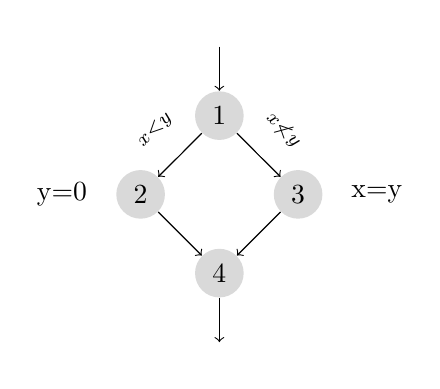
\begin{tikzpicture}
 \node (entry) at (1,3) {};
 \node (exit) at (1,-1) {};
 \node (text1) at (-1,1) {y=0};
 \node (text2) at (3,1) {x=y};
 \tikzstyle{every node} = [circle,fill=gray!30]
 \node (a) at (1,2) {1};
 \node (b) at (0,1) {2};
 \node (c) at (2,1) {3};
 \node (d) at (1,0) {4};
 \draw [->] (entry) to (a);
 \draw [->] (a)  -- node[color=black,fill=white,pos=0.5,sloped,above] {$
   \scriptstyle x<y$} (b);
 \draw [->] (a)  -- node[color=black,fill=white,pos=0.5,sloped,above]
 {$\scriptstyle x \not <
   y$} (c);
 \draw [->] (c) to (d);
 \draw [->] (b) to (d);
 \draw [->] (d) to (exit);
\end{tikzpicture}
\end{column}
\end{columns}
\end{frame}

\begin{frame}[fragile]%{If statement}
\frametitle{If statements}
\begin{columns}
\begin{column}{0.5\textwidth}
\begin{lstlisting}
         if (x<y) 
         { 
           y=0; 
         };

\end{lstlisting}
\end{column}
\begin{column}{0.5\textwidth}
 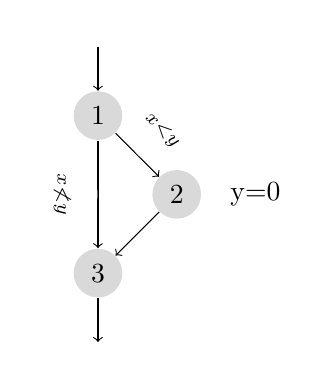
\begin{tikzpicture}
 \node (entry) at (1,3) {};
 \node (exit) at (1,-1) {};
 \node (text2) at (3,1) {y=0};
 \tikzstyle{every node} = [circle,fill=gray!30]
 \node (a) at (1,2) {1};
 \node (c) at (2,1) {2};
 \node (d) at (1,0) {3};
 \draw [->] (entry) to (a);
 \draw [->] (a)  -- node[color=black,fill=white,pos=0.5,sloped,above] {$
   \scriptstyle x<y$} (c);
 \draw [->] (a)  -- node[color=black,fill=white,pos=0.5,sloped,below]
 {$\scriptstyle x \not <
   y$} (d);
 \draw [->] (c) to (d);
 \draw [->] (d) to (exit);
\end{tikzpicture}
\end{column}
\end{columns}
\end{frame}

\begin{frame}[fragile]%{If statement}
\frametitle{If return statements}
\begin{columns}
\begin{column}{0.5\textwidth}
\begin{lstlisting}
         if (x<y) 
         { 
           return;
         }
         print(x);
         return;
\end{lstlisting}
\end{column}
\begin{column}{0.5\textwidth}
 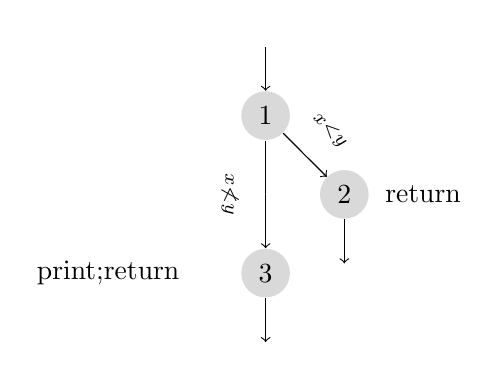
\begin{tikzpicture}
 \node (entry) at (1,3) {};
 \node (exit) at (1,-1) {};
 \node (exit2) at (2,0) {};
 \node (text2) at (3,1) {return};
 \node (text3) at (-1,0) {print;return};
 \tikzstyle{every node} = [circle,fill=gray!30]
 \node (a) at (1,2) {1};
 \node (c) at (2,1) {2};
 \node (d) at (1,0) {3};
 \draw [->] (entry) to (a);
 \draw [->] (a)  -- node[color=black,fill=white,pos=0.5,sloped,above] {$
   \scriptstyle x<y$} (c);
 \draw [->] (a)  -- node[color=black,fill=white,pos=0.5,sloped,below]
 {$\scriptstyle x \not <
   y$} (d);
 \draw [->] (d) to (exit);
 \draw [->] (c) to (exit2);
\end{tikzpicture}
\end{column}
\end{columns}
Note that we do not collapse the two return statements. 
\end{frame}

\begin{frame}[fragile]{Loops}
\begin{columns}
\begin{column}{0.5\textwidth}
\begin{lstlisting}
  for(i=0; i<x; i++) {
    loop_body();
  }
\end{lstlisting}
\end{column}
\begin{column}{0.5\textwidth}
 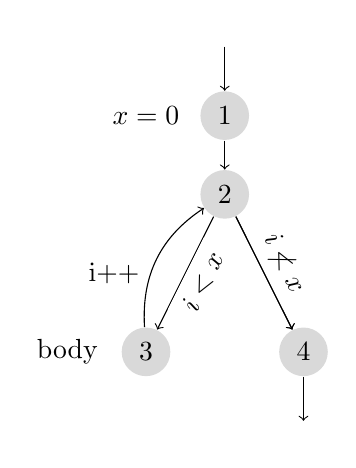
\begin{tikzpicture}
 \node (entry) at (1,3) {};
 
% \tikzstyle{every node} = [circle,fill=gray!30]
 \node[below of=entry,circle,fill=gray!30] (initialise) {$1$};
 \node[left  of=initialise] () {$x=0$};
 \node[below of=initialise,circle,fill=gray!30] (start) {$2$};
 \node[below of=start] (placementnode) {};
 \node[left of=placementnode, below of=placementnode,circle,fill=gray!30] (body)
 {$3$}; 
 \node[left of=body] () {body};
 \node[left of=placementnode,node distance=4em] (anchorpoint) {i++};
 \node[right of=placementnode, below of=placementnode,circle,fill=gray!30] (exit)
{$4$};
 \node[below of=exit] (exitnode) {};
 
 \draw [->] (exit) to (exitnode);
 \draw [->] (entry) to (initialise);
 \draw [->] (initialise) to (start);
 \draw [->] (start) --
 node[color=black,fill=white,pos=0.5,below,sloped] {$\scriptsize i<x$}
 (body);
 \draw [->] (start) --
 node[color=black,fill=white,pos=0.5,above,sloped] {$\scriptsize i\not<x$} (exit);
 \draw [->] (start) to (exit);
  \draw [->] (body) to[bend left] (start);
\end{tikzpicture}
\end{column}
\end{columns}
\end{frame}

\begin{frame}
  \begin{itemize}
  \item Other program constructs are easy to do.
  \item Each node is only to be labelled with one basic block.
  \item Beware of hidden control structures. (C's case statement).
  \end{itemize}
\end{frame}
 \begin{frame}{Paths}
Other possible definitions.
   \begin{itemize}
   \item A path is a sequence of nodes.
   \item The length of a path is the number of edges. A path with only
     one node, hence no edge has length $0$.
   \item Subpath is sub-sequence of a path.
   \item $\Reach(n)$  the set of nodes that can be reach via  a
     directed path from the node $n$.
   \end{itemize}
 \end{frame}

 \begin{frame}{Paths}
       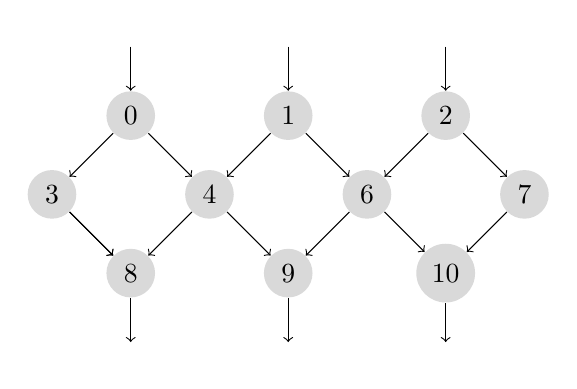
\begin{tikzpicture}
         \node (entry1) at (1,3) {} ;
     \node (entry2) at (3,3) {} ;
     \node (entry3) at (5,3) {};
     \node (exit1) at (1,-1) {} ;
     \node (exit2) at (3,-1) {} ;
     \node (exit3) at (5,-1) {} ;
     \tikzstyle{every node} = [circle,fill=gray!30]
     \node (a1) at (1,2) {0};
     \node (a2) at (3,2) {1};
     \node (a3) at (5,2) {2};
     \node (b1) at (0,1) {3};
     \node (b2) at (2,1) {4};
     \node (c2) at (4,1) {6};
     \node (c3) at (6,1) {7};
     \node (d1) at (1,0) {8};
     \node (d2) at (3,0) {9};
     \node (d3) at (5,0) {10};
     \draw [->] (entry1) to (a1);
     \draw [->] (entry2) to (a2);
     \draw [->] (entry3) to (a3);
     \draw [->] (a1) to (b1);
     \draw [->] (a1) to (b2);
     \draw [->] (b2) to (d1);
     \draw [->] (b1) to (d1);
     \draw [->] (b1) to (d1);
     \draw [->] (d1) to (exit1);
     \draw [->] (a2) to (b2);
     \draw [->] (a2) to (c2);
     \draw [->] (c2) to (d2);
     \draw [->] (b2) to (d2);
     \draw [->] (d2) to (exit2);
     \draw [->] (a3) to (c2);
     \draw [->] (a3) to (c3);
     \draw [->] (c3) to (d3);
     \draw [->] (c2) to (d3);
     \draw [->] (d3) to (exit3);
   \end{tikzpicture}
   \begin{itemize}
   \item Paths include: $[0,3,8],[0,4,8],[0,4,9],[1,4,8],\ldots ,
     [4,8], \ldots$.
   \end{itemize}
 \end{frame}
 \begin{frame}{$\Reach(n)$}
       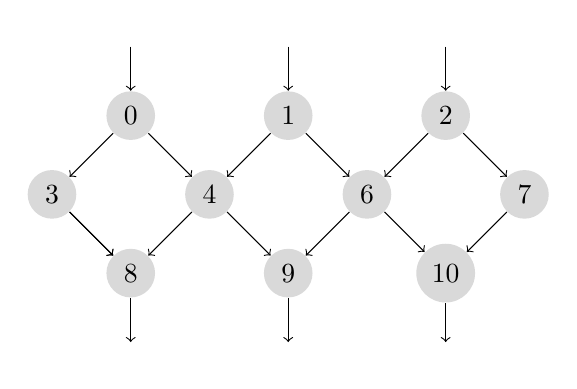
\begin{tikzpicture}
         \node (entry1) at (1,3) {} ;
     \node (entry2) at (3,3) {} ;
     \node (entry3) at (5,3) {};
     \node (exit1) at (1,-1) {} ;
     \node (exit2) at (3,-1) {} ;
     \node (exit3) at (5,-1) {} ;
     \tikzstyle{every node} = [circle,fill=gray!30]
     \node (a1) at (1,2) {0};
     \node (a2) at (3,2) {1};
     \node (a3) at (5,2) {2};
     \node (b1) at (0,1) {3};
     \node (b2) at (2,1) {4};
     \node (c2) at (4,1) {6};
     \node (c3) at (6,1) {7};
     \node (d1) at (1,0) {8};
     \node (d2) at (3,0) {9};
     \node (d3) at (5,0) {10};
     \draw [->] (entry1) to (a1);
     \draw [->] (entry2) to (a2);
     \draw [->] (entry3) to (a3);
     \draw [->] (a1) to (b1);
     \draw [->] (a1) to (b2);
     \draw [->] (b2) to (d1);
     \draw [->] (b1) to (d1);
     \draw [->] (b1) to (d1);
     \draw [->] (d1) to (exit1);
     \draw [->] (a2) to (b2);
     \draw [->] (a2) to (c2);
     \draw [->] (c2) to (d2);
     \draw [->] (b2) to (d2);
     \draw [->] (d2) to (exit2);
     \draw [->] (a3) to (c2);
     \draw [->] (a3) to (c3);
     \draw [->] (c3) to (d3);
     \draw [->] (c2) to (d3);
     \draw [->] (d3) to (exit3);
   \end{tikzpicture}   
   \begin{itemize}
   \item $\Reach(3) = \{8\}$, $\Reach(1) = \{4,9,8,6,10\}$.
   \end{itemize}
 \end{frame}
%%%%%%%%
\begin{frame}[fragile]{Reach}
  \begin{itemize}
  \item Two notions in program analysis:
    \begin{itemize}
    \item Syntactic Reach. 
    \item Semantic Reach.
    \end{itemize}
   \end{itemize}
\begin{lstlisting}
      main() {
        for(i=0; true; i++) {
          if (f(i) == 0) { break(0);}
        }
        X();
      }
\end{lstlisting}
%%%
{\tt X()}  is syntactically reachable, but
semantically you have to infer something about {\tt f()}.
\end{frame}
%%%%%%%
\begin{frame}{Test Path}
   \begin{itemize}
   \item  A test path starts at an initial node and ends in a final
     node.
   \item Test paths represent execution of test cases.
     \begin{itemize}
     \item  Some paths can be executed by many test cases.
     \item Some paths can not be executed by any test cases (halting
       problem again).
     \end{itemize}
   \end{itemize}
\end{frame}
%%%%%%%
 \begin{frame}{Test Cases and Test Paths}
\begin{center}
   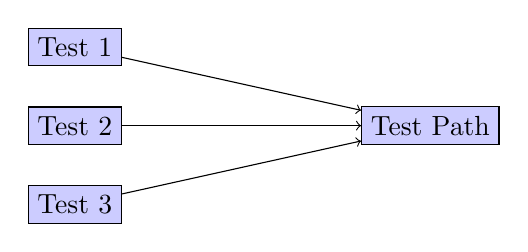
\begin{tikzpicture}
     \node[rectangle,draw,fill=blue!20] (test1) {Test 1};
     \node[rectangle,below of=test1,draw,fill=blue!20] (test2) {Test 2};
     \node[rectangle,below of=test2,draw,fill=blue!20] (test3) {Test
       3};
     \node[right of=test2,node distance=10em]  (placementnode) {};
     \node[rectangle,right of=placementnode,draw,fill=blue!20] (path)
     {Test Path};
     \draw [->] (test1) to (path);
     \draw [->] (test2) to (path);
     \draw [->] (test3) to (path);
   \end{tikzpicture}
\end{center}
Many to one. Deterministic software, each test path has identical
execution.
\begin{center}
   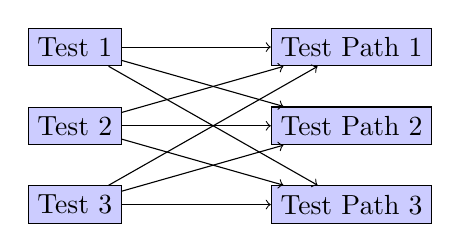
\begin{tikzpicture}
     \node[rectangle,draw,fill=blue!20] (test1) {Test 1};
     \node[rectangle,below of=test1,draw,fill=blue!20] (test2) {Test 2};
     \node[rectangle,below of=test2,draw,fill=blue!20] (test3) {Test
       3};
     \node[rectangle,right of=test1,draw,fill=blue!20,node
     distance=10em] (path1) {Test Path 1};
     \node[rectangle,right of=test2,draw,fill=blue!20,node
          distance=10em] (path2) {Test Path 2};
     \node[rectangle,right of=test3,draw,fill=blue!20,node
     distance=10em] (path3) {Test Path 3};
     \draw[->] (test1) to (path1);
     \draw[->] (test1) to (path2);
     \draw[->] (test1) to (path3);
     \draw[->] (test2) to (path1);
     \draw[->] (test2) to (path2);
     \draw[->] (test2) to (path3);
     \draw[->] (test3) to (path1);
     \draw[->] (test3) to (path2);
     \draw[->] (test3) to (path3);
   \end{tikzpicture}
\end{center}
Many to many, non-deterministic software (you'll meet it all the time)
a test can execute many test paths.
\end{frame}
\begin{frame}{Thinking about testing}
  Important to separate:
  \begin{itemize}
  \item What coverage criteria are we trying to test?
    \begin{itemize}
    \item Branch, statement, function points $\ldots$
    \end{itemize}
  \item How do we test this property?
    \begin{itemize}
    \item What paths do we cover in the control flow graph?
    \end{itemize}
    \item What test cases (inputs and expected outputs) will make the
      paths execute? 
  \end{itemize}
\end{frame}



\begin{frame}
  \frametitle{Summary}
  \begin{itemize}
  \item Turing's halting theorem tells us that in a strong sense that testing
    for correctness is impossible.
  \item Formalising programs as control flow graphs gives us a way to talk
    about testing.
  \item Node coverage corresponds to statement coverage, edge coverage
    corresponds to something like branch coverage. Covering all execution
    paths is impossible with loops, so there are various approximations.
  \end{itemize}
  Don't forget the distinction between syntactic and semantic reachability. 
\end{frame}

\end{document}

%%% Local Variables:
%%% mode: latex
%%% TeX-master: t
%%% End:
